\chapter{Traditional models}
\label{ch:TM}

To estimate a PD model, different types of models varying in complexity are available:

\begin{enumerate}
  \item Statistical Models: This type utilizes historical data for the estimation process. Techniques such as logistic regression and machine learning algorithms are used to predict default events and analyze contributing risk factors.
  \item External Rating Models: Rating agencies develop models that assign credit ratings to borrowers. These models consider various factors, e.g., financial statements and macroeconomic conditions, to evaluate creditworthiness. These types of PD models are only available for a limited portion of borrowers. 
  \item Expert Judgment: In cases where historical data is limited or only a low number of default events is available, expert judgment will become the most relevant method. Experienced credit analysts rely on their expertise and industry knowledge to estimate the PD based on qualitative factors, market conditions and client information.
\end{enumerate}

In practice, a substantial portion of the banking sector employs a combination of multiple types of models in their credit risk assessment.

\section{Logistic regression}
Logistic regression is one of the banking industry's most commonly used statistical models. In the logit model, the log odds are modeled as a linear function, given in Equation \ref{eq:tm_logodds}. The right side, also called the linear predictor, results in a model score, which can take any negative or positive value. Equation \ref{eq:tm_logodds} can be re-formulated to calculate the \ac{PD}, yielding Equation \ref{eq:tm_prob}, which presents the logistic function that confines the probability from 0 to 1. Therefore, a high model score means a lower \ac{PD} and vice versa.\footnote{\cite{Kuhn:2013} p.~283}

\begin{figure}[H]
\begin{minipage}{.5\textwidth}
	\begin{align}
	log (\frac{PD}{1 - PD}) = \sum_{i=1}^{n} \beta_{0} + \beta_{i} \times x_i \label{eq:tm_logodds}\\
	PD = \frac{1}{1 + e^{-(\sum_{i=1}^{n} \beta_{0} + \beta_{i} \times x_i)}} \label{eq:tm_prob}
	\end{align}
\end{minipage}%
\begin{minipage}{.5\textwidth}
	\centering
	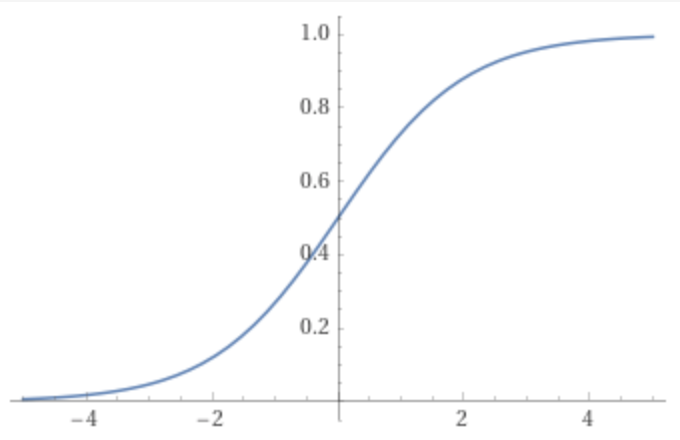
\includegraphics[width=.5\textwidth]{./TM__logistic_func.png}
\end{minipage}
    \caption{Logistic Function}
    \label{fig:tm_logfunc}
\end{figure}

\section{Other Models}

\subsection{Linear regression}
During the linear regression, the algorithm estimates a linear relationship between the default variable, which assumes either the value 0 (non-default) or 1 (default), and explanatory variables, which can be continuous and categorical independent variables, such as income, employment duration and profession. In ordinary least squares linear regression, the goal is to minimize the sum of squared differences between observed and predicted values, with model coefficients determined by Equation \ref{eq:tm_linreg}. The minimization problem is successful, if all explanatory variables are linear independent and thus, the correlation between variables has to be reduced. Disadvantages of this method are that the model may output non-logical results, like negative values or a PD over 100\%, and its limitation in capturing non-linear relationships.\footnote{\cite{Kuhn:2013} pp.~105, 108-109}

\vspace{-0.5cm}
\begin{equation}
\hat{\beta} = (X^T X)^{-1} X^T y \label{eq:tm_linreg}
\end{equation}
where:
\vspace{-0.5cm}
\begin{conditions}
\hat{\beta} & Vector of model coefficients \\
X & Matrix of explanatory variables \\
y & Vector of default variable
\end{conditions}

\vspace{-1cm}
\subsection{External Ratings}
Scorings of corporate clients are usually performed mainly by a credit analyst and only partly automated due to the low number of default events and the type of information available. External ratings may be used if the financial institution needs more resources to develop and maintain internal models. The most known rating agencies are Standard \& Poor, Moody's and Fitch. They provide ratings for a wide range of corporations since most companies request a rating before a sale or registration of a debt issue. 

An analyst will use their financial statements of the last few years and additional information to derive a rating, which is then discussed in a rating committee. Afterward, the corporation is informed about its rating and the corresponding factors and given the opportunity to respond; finally, the ratings will be published. A disadvantage of external ratings observed in the past is the conflict of interest since the company mainly pays the ratings. It is suspected that good ratings were related to high fees, which was visible during the financial crisis, where many structured bonds with high scorings deteriorated unexpectedly.\footnote{\cite{Witzany:2017} pp.~34-36}